\documentclass[tikz,border=5pt]{standalone}
\usepackage{tikz}
\usepackage{amsmath}
\usetikzlibrary{positioning,shapes,arrows.meta,calc,fit,backgrounds}

\definecolor{parentBlue}{HTML}{2E86AB}
\definecolor{childRed}{HTML}{C73E1D}
\definecolor{precisionGreen}{HTML}{4CAF50}
\definecolor{recallOrange}{HTML}{FF9800}
\definecolor{bgLight}{HTML}{F5F5F5}

\begin{document}
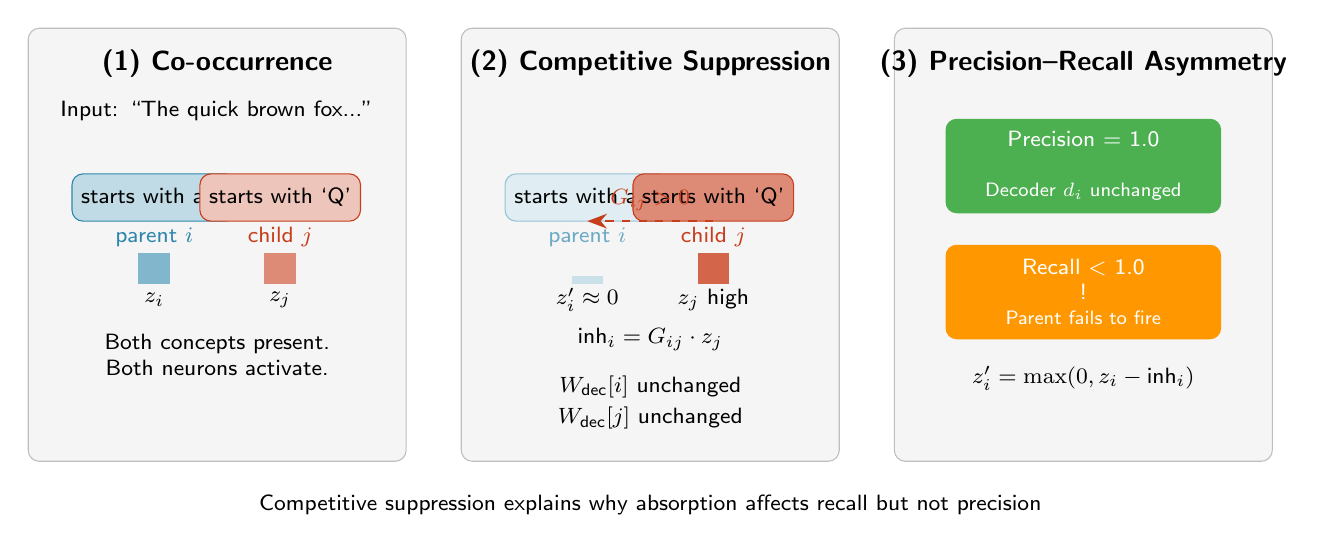
\begin{tikzpicture}[
    font=\sffamily\small,
    panel/.style={draw=gray!50, rounded corners, minimum width=4.8cm, minimum height=5.5cm},
    neuron/.style={rectangle, rounded corners, draw, minimum width=2cm, minimum height=0.6cm, align=center},
    bar/.style={rectangle, draw, minimum width=0.35cm},
    arrow/.style={-{Stealth[length=2.5mm]}, thick},
    labelText/.style={font=\sffamily\footnotesize}
]

% === Panel 1: Co-occurrence ===
\node[panel, fill=bgLight] (p1) at (-5.5, 0) {};
\node[labelText, font=\sffamily\bfseries] at (-5.5, 2.3) {(1) Co-occurrence};

% Input text
\node[labelText, align=center] at (-5.5, 1.7) {Input: ``The quick brown fox...''};

% Parent neuron
\node[neuron, fill=parentBlue!30, draw=parentBlue] (p1_parent) at (-6.3, 0.6) {\footnotesize starts with any};
\node[labelText, parentBlue] at (-6.3, 0.1) {parent $i$};

% Child neuron
\node[neuron, fill=childRed!30, draw=childRed] at (-4.7, 0.6) {\footnotesize starts with `Q'};
\node[labelText, childRed] at (-4.7, 0.1) {child $j$};

% Activation bars - equal height
\fill[parentBlue!60] (-6.5, -0.5) rectangle (-6.1, -0.1);
\fill[childRed!60] (-4.9, -0.5) rectangle (-4.5, -0.1);
\node[labelText] at (-6.3, -0.7) {$z_i$};
\node[labelText] at (-4.7, -0.7) {$z_j$};

% Label
\node[labelText, align=center] at (-5.5, -1.4) {Both concepts present.\\Both neurons activate.};

% === Panel 2: Competitive Suppression ===
\node[panel, fill=bgLight] (p2) at (0, 0) {};
\node[labelText, font=\sffamily\bfseries] at (0, 2.3) {(2) Competitive Suppression};

% Parent neuron (dimmed)
\node[neuron, fill=parentBlue!15, draw=parentBlue!50] (p2_parent) at (-0.8, 0.6) {\footnotesize starts with any};
\node[labelText, parentBlue!70] at (-0.8, 0.1) {parent $i$};

% Child neuron (bright)
\node[neuron, fill=childRed!60, draw=childRed] (p2_child) at (0.8, 0.6) {\footnotesize starts with `Q'};
\node[labelText, childRed] at (0.8, 0.1) {child $j$};

% Inhibition arrow
\draw[arrow, childRed, dashed] (0.8, 0.3) -- node[above, labelText, childRed] {$G_{ij} > 0$} (-0.8, 0.3);

% Activation bars - parent low, child high
\fill[parentBlue!25] (-1.0, -0.5) rectangle (-0.6, -0.4);
\fill[childRed!80] (0.6, -0.5) rectangle (1.0, -0.1);
\node[labelText] at (-0.8, -0.7) {$z_i' \approx 0$};
\node[labelText] at (0.8, -0.7) {$z_j$ high};

% Equation
\node[labelText, align=center] at (0, -1.2) {$\text{inh}_i = G_{ij} \cdot z_j$};

% Decoder directions preserved
\node[labelText, align=center] at (0, -1.8) {\footnotesize $W_{\text{dec}}[i]$ unchanged};
\node[labelText, align=center] at (0, -2.2) {\footnotesize $W_{\text{dec}}[j]$ unchanged};

% === Panel 3: Precision-Recall Asymmetry ===
\node[panel, fill=bgLight] (p3) at (5.5, 0) {};
\node[labelText, font=\sffamily\bfseries] at (5.5, 2.3) {(3) Precision--Recall Asymmetry};

% Precision box
\node[rectangle, rounded corners, fill=precisionGreen, text=white, minimum width=3.5cm, minimum height=1.2cm, align=center] (prec) at (5.5, 1.0) {\footnotesize Precision = 1.0\\[-2pt]\footnotesize $\checkmark$\\[-2pt]\scriptsize Decoder $d_i$ unchanged};

% Recall box
\node[rectangle, rounded corners, fill=recallOrange, text=white, minimum width=3.5cm, minimum height=1.2cm, align=center] (rec) at (5.5, -0.6) {\footnotesize Recall $<$ 1.0\\[-2pt]\footnotesize !\\[-2pt]\scriptsize Parent fails to fire};

% Equation
\node[labelText, align=center] at (5.5, -1.7) {$z_i' = \max(0, z_i - \text{inh}_i)$};

% === Bottom annotation ===
\node[labelText, font=\sffamily\footnotesize, align=center] at (0, -3.3) {Competitive suppression explains why absorption affects recall but not precision};

\end{tikzpicture}
\end{document}
